\subsection{A* Search with heuristic}
\noindent A* algorithm is one of the popular technique used in path finding and graph traversals. This algorithm completely relies on heuristics for computing the future cost of a problem. This algorithm is equivalent to the uniform cost search with modified edge cost. This heuristics is chosen according to the case where the algorithm is implemented, thus emphasizing the importance of domain knowledge. This algorithm is consistent if the modified cost is greater than zero.

\begin{figure}[H]
	\centering
	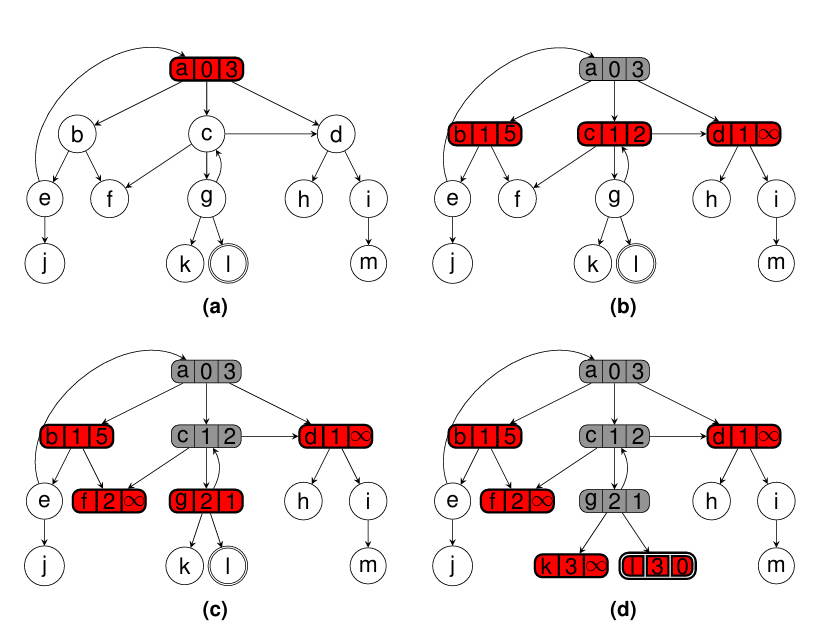
\includegraphics[width=0.8\textwidth]{./imgs/astar.png}
	\caption{A* Algorithm}
\end{figure}

\subsubsection{Pseudocode}
\begin{algorithm}[H]
	\caption{A* Search (\textit{start, goal, heuristic})}
	\label{alg:astar}
	\begin{algorithmic}[1]
		\State priority queue \(\gets\) [(start, cost = 0, estimated total cost = heuristic(start))]
		\While {priority queue is not empty}
		\State (node, cost) \(\gets\) dequeue(priority queue)
		\If {node = goal}
		\State return path
		\EndIf
		\ForAll {neighbor in valid moves}
		\State new cost \(\gets\) cost + move cost
		\State estimated total cost \(\gets\) new cost + heuristic(neighbor)
		\If {neighbor not visited or new cost \(<\) previous cost}
		\State mark neighbor as visited
		\State enqueue(priority queue, (neighbor, new cost, estimated total cost))
		\EndIf
		\EndFor
		\EndWhile
		\State return failure
	\end{algorithmic}
\end{algorithm}

\subsubsection{Implementation}
\begin{itemize}
	\item \textbf{\_\_init\_\_(\ldots)}
	      Initializes the A* search algorithm with grid dimensions, matrix representation, initial player position, stone positions, and switch positions. It also includes options for deadlock detection and heuristic optimization.

	\item \textbf{search()}
	      Implements the A* search algorithm using a priority queue (min-heap). The function explores states by selecting the one with the lowest cost \(f = g + h\). It expands nodes by generating successors, updating costs, and maintaining a hash table for efficient state lookup.

	\item \textbf{handle(new\_state, closed, frontier, state\_hash\_table)}
	      Manages newly generated states, checking if they should be added to the frontier or updated in the hash table based on their cost values.

	\item \textbf{heuristic(stones\_pos, switches\_pos)}
	      Computes the heuristic function to estimate the cost to reach the goal. It selects between the Hungarian heuristic and Manhattan heuristic based on the optimization flag.

	\item \textbf{mahattan\_heuristic(stones\_pos, switches\_pos)}
	      Calculates the heuristic using the Manhattan distance, summing up the minimum distances from each stone to a switch.

	\item \textbf{hungarian\_heuristic(stones\_pos, switches\_pos)}
	      Uses the Hungarian algorithm to optimally assign stones to switches, minimizing the total weighted Manhattan distance.

	\item \textbf{can\_go(current\_state, dir)}
	      Checks whether the player can move in a given direction from the current state without encountering obstacles.

	\item \textbf{go(current\_state, dir, heuristic)}
	      Generates a new state by moving the player in the specified direction, updating positions and recalculating heuristic values.

	\item \textbf{construct\_path(final\_state)}
	      Reconstructs the sequence of moves leading to the goal state by backtracking from the final state.

\end{itemize}

\subsubsection{Time and Space Complexity}
\textbf{Time Complexity:} \( O(b^d) \) in the worst case, but with a good heuristic, it can be significantly reduced. If the heuristic is admissible and consistent, A* is optimal and complete.

\textbf{Space Complexity:} \( O(b^d) \), as it keeps all generated nodes in memory.
